\chapter{31. Schelling segregation model}

\resp{Jules Vandendriessche}



\section{Introduction to segregation}


This task focuses on an idea first introduced in 1973 by Schelling \cite{shelling}.  In this model, a slight aversion to dissimilar agents may lead to drastic segregation.  This model will be implemented 3 times in this task, each time adapted according to the proposed paper.

The original model proposed by shelling can be viewed as N people sitting on a 1-D line next to each other (this analogy because agents are for now free to place themselves anywhere freely). The agents have a property, that distinguishes the population in 2 groups. The neighbourhood exists out of the agents that affect an agent in question. In this analogy, it would be the agent left and right of it, however the neighbourhood can be extended. The  agents are happy when the fraction of similar neighbours in their neighbourhood is above the threshold ($f$), which is usually taken as $1/2$. However,  for now the threshold will be defined as the number of dissimilar agents in the neighbourhood that are tolerated.  The dynamics of this first case goes as follows: An unhappy agent is selected at random, and it looks for the closest positions in between other agents where it will be happy.  If there is no position where his wishes are satisfied, he will lower his threshold by one and try again. If it is still not possible, he prefers to not move and will remain unhappy.
This  goes on until an equilibrium stage has been reached.
For this part, null boundaries are considered, meaning that agents on the ends only have 1 neighbor.

In the paper written by D'all'Asta et al \cite{Dall’Asta_2008}, some changes to the dynamics are proposed. First of  all, empty sites are introduced, hence the analogy to a 1-D street with houses and agents that move in between them is of order. Agents are free to move to any house (empty site) that fulfils their needs. Furthermore we will take a look  at an unconstrained model, where agents are allowed to move as long as their utility does not decrease. Lastly, a comparison is made between non binary and binary dynamics. Meaning that agents who have  a neighbourhood filled with agents that are alike, and agents that have a neighbourhood just above the threshold will be distinguished in the non binary case, and viewed as the same in the binary case. The threshold (f) is now defined as the magnetisation of the agents neighbourhood multiplied by the spinstate of the agent. Periodic boundaries are considered in this case.

The third paper by Henry et.al \cite{adam} introduces agents on a network. Agents have a certain continuous property and they are connected through links, with a length defined according to the metric that is defined as:
\[
d_K(x, y, K) = \begin{cases}
\frac{1}{K} & \text{if } x = y, \\
\frac{\lceil K \cdot \frac{|x - y|}{2} \rceil}{K} & \text{if } x \neq y.
\end{cases}
\]

with x and y the property of the agent connected through the edge, and K a parameter such that only a certain amounts of lengths occur. K will be taken to be 4.
These links will be 'short' if it connects similar agents, and will be 'long' if it connects dissimilar agents. At each turn an edge is selected and will be cut with a probability related to the length of that edge. If cut, the agent will form a link with a random agent. It can be proven, and we will show numerically, that the resulting length distribution of the links is independent on the initial network. 
 


\section{Results and discussion}
Regarding the simple model of Schelling's original model, one expects the same dynamics when the fraction $\frac{\text{neighbourhood}}{\text{threshold}}$ is the same. This is generally seen in Figure \ref{figuur2}. However, defining the magnetisation $\frac{N_+ - N_-}{N_+ + N_-}$, with $N_+$ and $N_-$ indicating the number of agents in each group and denoting the tuple (threshold, neighbourhood), one sees a dissimilarity between (1,2) and (2,4); the first being not segregated, the latter segregated. This relates to the phase space of happy configurations: -++ and ++- for (1,2) and --+++, -+++-, +++--, +-+-+, +-++-, and -++-+ for (2,4). Even though the agents are less stringent about the state of their neighbourhood, the dynamics produce a more segregated configuration.
Due to the additional rule of lowering the threshold, the result is an almost bi-diagonal matrix. Two exceptions are noted. When the magnetisation is too small with respect to the threshold, the minority is too sparsely distributed, and a configuration where an agent would be happy does not exist. Note that if cooperation is allowed, they could group together and be happy. Secondly, when the magnetisation is zero, the data matrix starts becoming tri-diagonal, indicating that segregation occurs even when agents are happy in a neighbourhood with more dissimilar agents.

Regarding the second paper, we'll first focus on the constrained model, meaning that the nodes only move when they are unhappy. The neighbourhood is defined as the two sites next to the agent. Spin states are used, with -1 and +1 indicating agents belonging to each group, and an empty site denoted by 0. Utility is defined as the sum of the states of the agent's neighbourhood. The empty site density, $p$, is defined as $\frac{N_0}{N_+ + N_- + N_0}$. Denote by $u$ the density of unhappy agents. In Figure \ref{figuur1}, $u$ is plotted against $m$ and $p$. Visualizing the figure, several points can be noted.
First, $u_\infty$ is supposed to vanish at $m=0$ and $m=1$ and for large enough $p$. This occurs because, as long as there is one empty site, nodes can gradually improve their utility, and a configuration where everybody is happy is always obtainable (assuming $m=0$). For $m=1$, by definition, there are no unhappy nodes. For large enough $p$, it vanishes because nodes, in the worst-case scenario, live on their own, which is a happy configuration when $f = 0$.
The reason for the peak in unhappiness is due to the decrease of the minority. The minority will be, on average, less satisfied the smaller it becomes, but this effect is negated by the increase in the happy majority. Hence, on average, more agents are happy.

In the analysis of unconstrained dynamics, a comparison is made between neighborhood sizes of 2 and 4, with the threshold set at zero and slightly above. This means that agents are happy if their neighborhood is equally split in the first case, and require a slight majority in the latter. This comparison is done for both binary (Figure \ref{figuur3}) and non-binary (Figure \ref{figuur4}) utility functions. The plots show how the dynamics of a random initial configuration evolves depending on the neighborhood and the threshold, in function of p. The density of unhappy agents and the density of interfaces (density of opposite spin-states neighboring each other) are also shown.
For the non-binary utility function, focusing on the highest values of p, it is seen that a larger neighborhood induces more segregation than a smaller neighborhood, similar to what was seen in Schelling's original model. A transition seems to happen in the case of the smaller neighborhood when pp increases. Local structures form but do not persist. Note also that segregation happens equally for all spin-states, in contrast to the binary utility function where segregation to opposite spin-states is seen, along with random patches of empty sites.
Taking our focus to the binary utility function and still looking at the high density of empty sites, segregation remains when the threshold is raised above 0. This is expected since the only happy state for a neighborhood of 2 would be +++, and for 4 it would be +++++, +-+++, and their permutations. In this latter case, the opposite spin would not be happy and would move. Furthermore, this raise in threshold can constrain the unconstrained model when the density of empty sites is too low.
Regarding the densities of unhappy agents and of interfaces, these converge rather fast, at about 100 iterations, after which they fluctuate, with 2 exceptions (Figure \ref{figuur4}, plot 2, p=[0.5,0.3]). In general, the higher the p, the faster the convergence. 
The oscillations are caused by agents moving to empty sites, lowering the magnetization of the neighborhood of their old neighbors.
In the case of smaller p, and as long as the dynamics are still unconstrained, complete segregation happens with a buffer of empty sites.


Regarding the third paper, a simulation is ran for 100 nodes, who have an attribute randomly sampled from U(-1,1). Four graph are used, of which Erdos-Renyi and Barabasi-Albert. The two other graphs are denoted as 'long links' (LL) and 'short links' (SL). The LL graphs connects all nodes if the corresponding edge would have maximal length, SL if minimal. At each time-step, a random edge is selected, and will be cut with probability $p\times length$, with $p\in (0,1]$. It is seen that convergence is faster, the higher p, but the end distribution does not depend on p. 



The general trend is found back, all four graphs their edge-length distributions converge to similar values. However, finite size effects are present, and the distributions are averaged over multiple realizations.


\section{Appendix}
\begin{figure}[H]
\begin{center}
	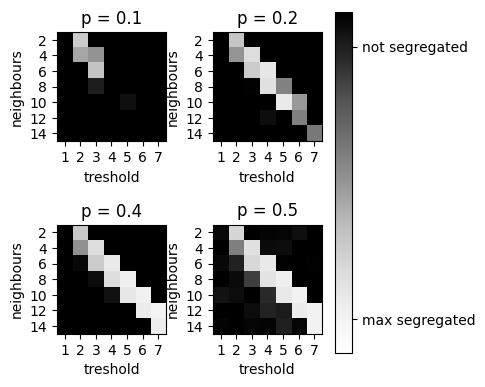
\includegraphics[width=0.6\textwidth]{fig2.png}
	\caption{\emph{ Segregation in function of threshold. Simulation done with 100 agents. Segregation scale is linear and normalised to minimal possible segregation (maximal possible groups) in system with given magnetisation. }}
	\label{figuur2}
\end{center}
\end{figure}



\begin{figure}[H]
\begin{center}
	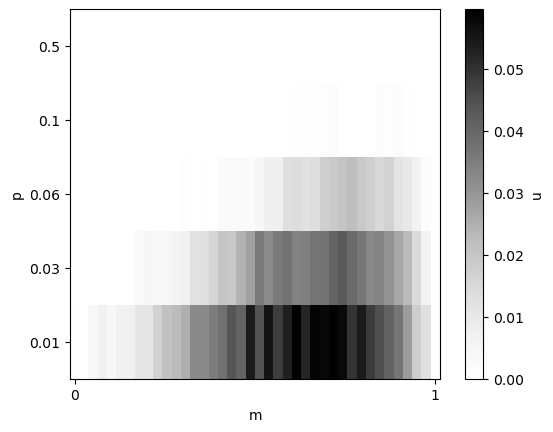
\includegraphics[width=0.5\textwidth]{fig1.png}
	\caption{\emph{ Density unhappy agents in function of m and p. 1000 agents are considered and averaged over 30 realisations. }}
	\label{figuur1}
\end{center}
\end{figure}



\begin{figure}[H]
\begin{center}
	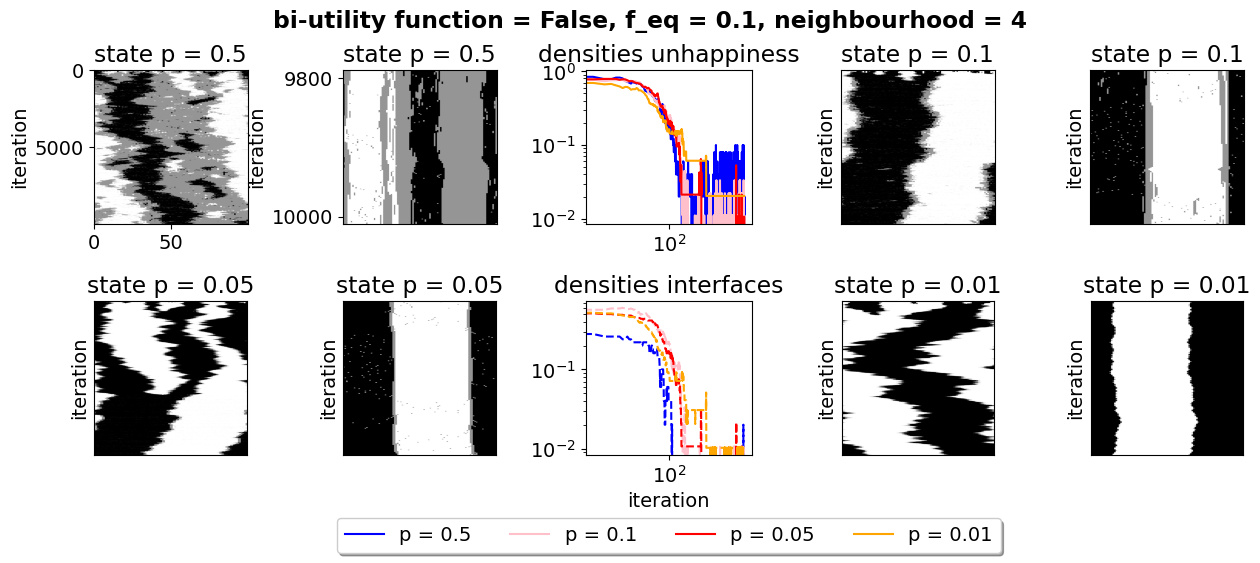
\includegraphics[width=0.8\textwidth]{dyn1.png}
	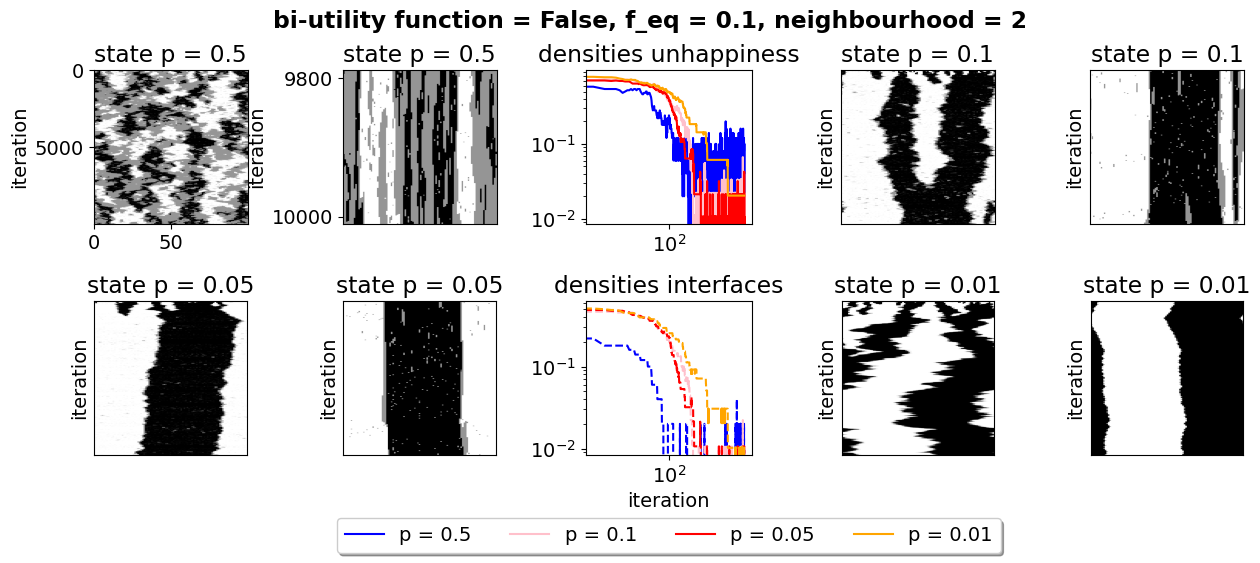
\includegraphics[width=0.8\textwidth]{dyn2.png}
	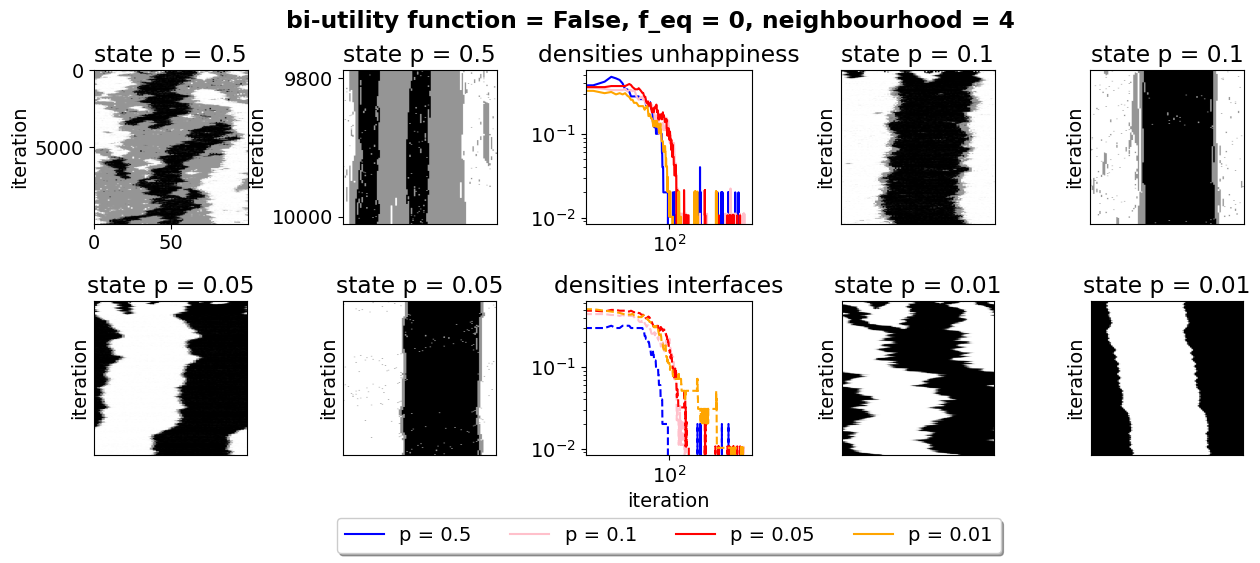
\includegraphics[width=0.8\textwidth]{dyn3.png}
	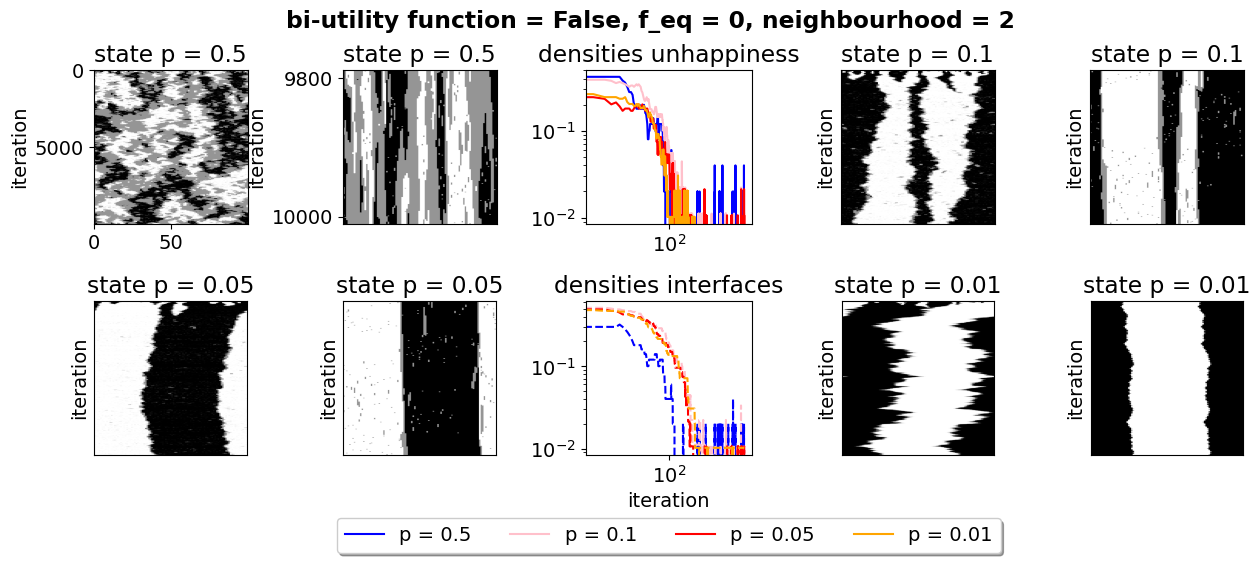
\includegraphics[width=0.8\textwidth]{dyn4.png}
 
	\caption{\emph{ Dynamics according to unconstrained model in function of threshold ($f_{eq}$) and size neighbourhood for non binary utility function. }}
	\label{figuur3}
\end{center}
\end{figure}

\begin{figure}[H]
\begin{center}
	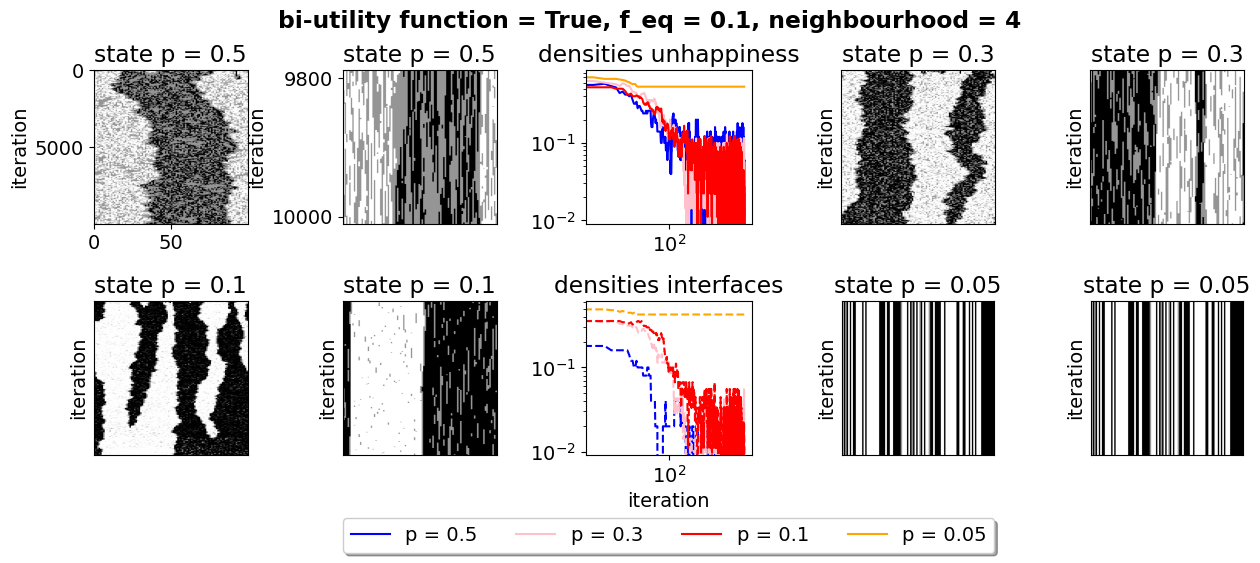
\includegraphics[width=0.8\textwidth]{dyn5.png}
	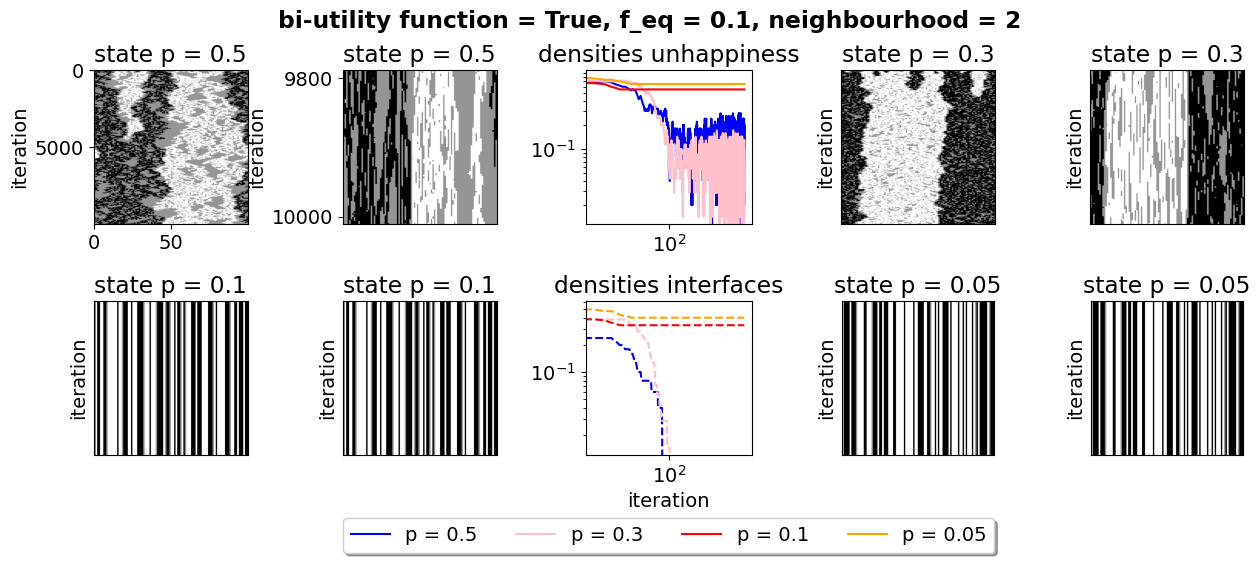
\includegraphics[width=0.8\textwidth]{dyn6.png}
	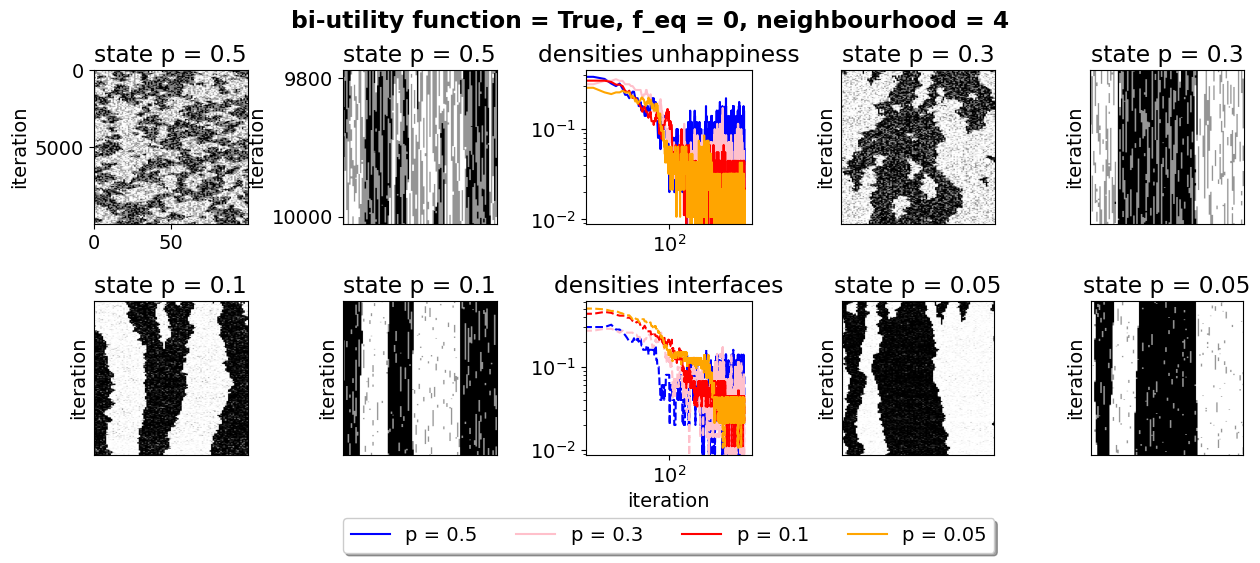
\includegraphics[width=0.8\textwidth]{dyn7.png}
	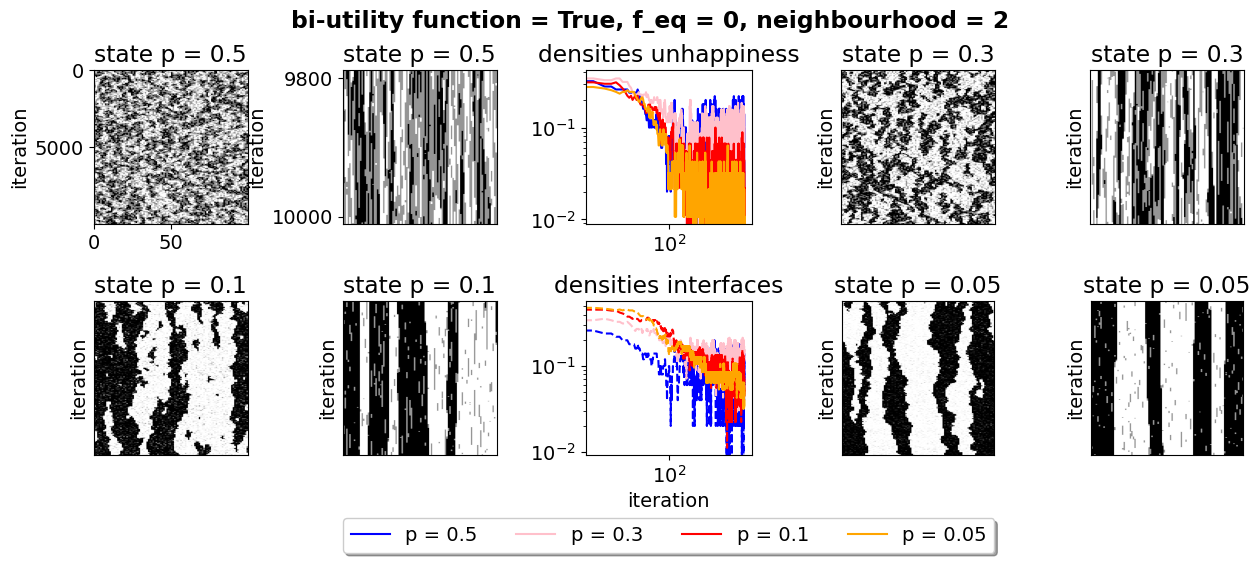
\includegraphics[width=0.8\textwidth]{dyn8.png}
 
	\caption{\emph{ Dynamics according to unconstrained model in function of threshold ($f_{eq}$) and size neighbourhood for  binary utility function. }}
	\label{figuur4}
\end{center}
\end{figure}

\newpage